\documentclass[tikz,border=4pt]{standalone}
\begin{document}
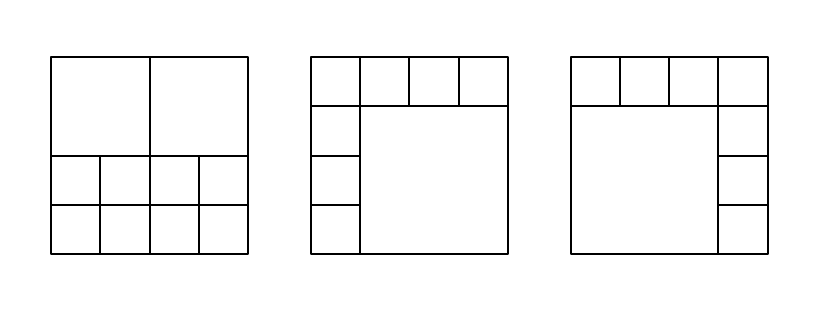
\begin{tikzpicture}[x=0.025cm,y=-0.025cm]
\path[use as bounding box] (0,0) rectangle (390,130);
\path[draw=black,fill=white,line width=0.72pt,line join=round] (12,15) -- (62,15) -- (62,65) -- (12,65) -- cycle;
\path[draw=black,fill=white,line width=0.72pt,line join=round] (62,15) -- (112,15) -- (112,65) -- (62,65) -- cycle;
\path[draw=black,fill=white,line width=0.72pt,line join=round] (12,65) -- (37,65) -- (37,90) -- (12,90) -- cycle;
\path[draw=black,fill=white,line width=0.72pt,line join=round] (37,65) -- (62,65) -- (62,90) -- (37,90) -- cycle;
\path[draw=black,fill=white,line width=0.72pt,line join=round] (62,65) -- (87,65) -- (87,90) -- (62,90) -- cycle;
\path[draw=black,fill=white,line width=0.72pt,line join=round] (87,65) -- (112,65) -- (112,90) -- (87,90) -- cycle;
\path[draw=black,fill=white,line width=0.72pt,line join=round] (12,90) -- (37,90) -- (37,115) -- (12,115) -- cycle;
\path[draw=black,fill=white,line width=0.72pt,line join=round] (37,90) -- (62,90) -- (62,115) -- (37,115) -- cycle;
\path[draw=black,fill=white,line width=0.72pt,line join=round] (62,90) -- (87,90) -- (87,115) -- (62,115) -- cycle;
\path[draw=black,fill=white,line width=0.72pt,line join=round] (87,90) -- (112,90) -- (112,115) -- (87,115) -- cycle;
\path[draw=black,fill=white,line width=0.72pt,line join=round] (169,40) -- (244,40) -- (244,115) -- (169,115) -- cycle;
\path[draw=black,fill=white,line width=0.72pt,line join=round] (144,15) -- (169,15) -- (169,40) -- (144,40) -- cycle;
\path[draw=black,fill=white,line width=0.72pt,line join=round] (169,15) -- (194,15) -- (194,40) -- (169,40) -- cycle;
\path[draw=black,fill=white,line width=0.72pt,line join=round] (194,15) -- (219,15) -- (219,40) -- (194,40) -- cycle;
\path[draw=black,fill=white,line width=0.72pt,line join=round] (219,15) -- (244,15) -- (244,40) -- (219,40) -- cycle;
\path[draw=black,fill=white,line width=0.72pt,line join=round] (144,40) -- (169,40) -- (169,65) -- (144,65) -- cycle;
\path[draw=black,fill=white,line width=0.72pt,line join=round] (144,65) -- (169,65) -- (169,90) -- (144,90) -- cycle;
\path[draw=black,fill=white,line width=0.72pt,line join=round] (144,90) -- (169,90) -- (169,115) -- (144,115) -- cycle;
\path[draw=black,fill=white,line width=0.72pt,line join=round] (276,40) -- (351,40) -- (351,115) -- (276,115) -- cycle;
\path[draw=black,fill=white,line width=0.72pt,line join=round] (276,15) -- (301,15) -- (301,40) -- (276,40) -- cycle;
\path[draw=black,fill=white,line width=0.72pt,line join=round] (301,15) -- (326,15) -- (326,40) -- (301,40) -- cycle;
\path[draw=black,fill=white,line width=0.72pt,line join=round] (326,15) -- (351,15) -- (351,40) -- (326,40) -- cycle;
\path[draw=black,fill=white,line width=0.72pt,line join=round] (351,15) -- (376,15) -- (376,40) -- (351,40) -- cycle;
\path[draw=black,fill=white,line width=0.72pt,line join=round] (351,40) -- (376,40) -- (376,65) -- (351,65) -- cycle;
\path[draw=black,fill=white,line width=0.72pt,line join=round] (351,65) -- (376,65) -- (376,90) -- (351,90) -- cycle;
\path[draw=black,fill=white,line width=0.72pt,line join=round] (351,90) -- (376,90) -- (376,115) -- (351,115) -- cycle;
\end{tikzpicture}
\end{document}
